\subsubsection{Router-Konfiguration}

\begin{figure}[H]
	\centering
	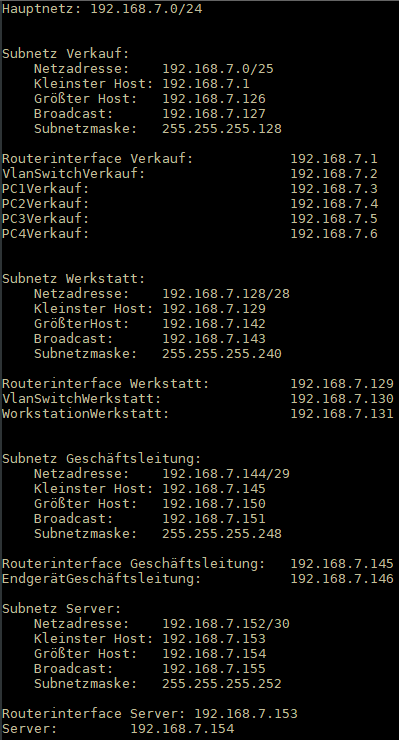
\includegraphics[width=7cm]{images/IPAdressen.png}
	\caption[Subnetze]{Subnetze mit zugeordneten IPs}
	\label{fig:subnetze}
\end{figure}

Bei der Router-Konfiguration wurde die IP-Addresskonfiguration am GigabitEthernet-Port 0/0/0 mit DHCP durchgeführt und als Default-Gateway der Standardgateway der EST gesetzt. Dem 
GigabitEthernet-Port 0/0/1 wurde eine statische IP-Adresse zugewiesen. Hierbei wurde die erste Host-IP innerhalb eines zuvor berechneten Subnetzes \ref{fig:subnetze} verwendet, um sich 
zumindest an die IP-Konfiguration des theoretischen Netzwerkes zu halten. Ebenso wurde eine Banner-Nachricht sowie Passwörter für den Konsolen-n Fern- und Konfigurationszugang 
vergeben. 

\subsubsection{Switch-Konfiguration}
Am Switch wurde ein VLAN-Interface eingerichtet,ebenfalls eine Banner-Nachricht und Passwörter für den Konsolen- und VLAN-Zugriff vergeben. An den beiden Kabelgebundenen Endgeräten 
wurde eine IP-Konfiguration die ebenfalls schonim Vorhinein geplant wurde, eingerichtet und die Firewall-Regeln wurden aktualisiert, um auf den Webserver, der auf einem der beiden 
Geräte gehostet wurde, zuzugreifen. 

\subsubsection{AP-Konfiguration}
Dem Access-Point wurde eine statische IP innerhalb des vorbestimmten Netzes zugewiesen und das Netzwerk mit WPA2 verschlüsselt. Da der Router nur mit statischen IP-Adressen
konfiguriert ist, ist auch eine Wireless-Verbindung nur dann möglich, wenn die IP-Adresse statisch eingestellt wird und sich innerhalb des Subnetzes des Access-Points befindet.

\subsubsection{Theoretische Gerätekonfiguration}
Die Konfigurationen der Geräte unterscheiden sich im Wesentlichen nicht von denen, die auch in der Praxis durchgeführt wurden. Es mussten nur zwei Switches statt einem und am Router vier
anstelle von zwei Ports konfiguriert werden. Die IP-Konfiguration war jedoch trotzdem dieselbe, die schon in \ref{fig:subnetze} dargestellt wurde.